\documentclass[12pt,letterpaper, margin = 3cm]{article}
\footskip = 50pt
\topmargin = -3cm
\usepackage[spanish]{babel}
%\usepackage[ansinew]{inputenc}
\usepackage[utf8]{inputenc}
% \usepackage[latin1]{inputenc}
\usepackage[letterpaper,includeheadfoot, top=0.5cm, bottom=5.0cm, right=2.0cm, left=2.0cm]{geometry}
\renewcommand{\familydefault}{\sfdefault}

\usepackage{graphicx}
\usepackage{color}
\usepackage{hyperref}
\usepackage{amssymb}
\usepackage{url}
%\usepackage{pdfpages}
\usepackage{fancyhdr}
\usepackage{hyperref}
\usepackage{subfig}

\usepackage{listings} %Codigo
\definecolor{dkgreen}{rgb}{0,0.6,0}
\definecolor{gray}{rgb}{0.5,0.5,0.5}
\definecolor{mauve}{rgb}{0.58,0,0.82}

\lstset{
  language=Java,
  aboveskip=3mm,
  belowskip=3mm,
  showstringspaces=false,
  columns=flexible,
  basicstyle={\small\ttfamily},
  numbers=none,
  numberstyle=\tiny\color{gray},
  keywordstyle=\color{mauve},
  commentstyle=\color{blue},
  stringstyle=\color{dkgreen},
  breaklines=true,
  breakatwhitespace=true
  tabsize=3
}

\begin{document}
%\begin{sf}
% --------------- ---------PORTADA --------------------------------------------
\newpage
\pagestyle{fancy}
\fancyhf{}
%-------------------- CABECERA ---------------------
\fancyhead[L]{ 
\includegraphics[scale=0.09]{img/logodcc.png} }
%------------------ TÍTULO -----------------------
\vspace*{5cm}
\begin{center}
\huge  {Tarea 2}\\
\Huge {KD-Trees}\\
\vspace{6cm}
\end{center}
%----------------- NOMBRES ------------------------
\vfill
\begin{flushright}
\begin{tabular}{ll}
Autores: & Claudio Berroeta\\
& Sebastián Ferrada \\
Profesor: & Pablo Barceló\\
Auxiliar: & Miguel Romero\\
Ayudantes: & Javiera Born\\
& Giselle Font\\
& \today\\
\end{tabular}
\end{flushright}

% ·············· ENCABEZADO - PIE DE PAGINA ············
\newpage
\pagestyle{fancy}
\fancyhf{}

%Encabezado
%\fancyhead[L]{\rightmark}
\fancyhead[L]{\small \rm \textit{Sección \rightmark}} %Izquierda
\fancyhead[R]{\small \rm \textbf{\thepage}} %Derecha


\fancyfoot[C]{\small \rm \textit{KD-Trees\\}} %Izquierda
%\fancyfoot[R]{\small \rm \textit{Pie de página - Derecha}} %Derecha
%\fancyfoot[C]{\thepage} %Centro

\renewcommand{\sectionmark}[1]{\markright{\thesection.\ #1}}
\renewcommand{\headrulewidth}{0.5pt}
\renewcommand{\footrulewidth}{0.5pt}
\newcommand{\fancyfootnotetext}[2]{%
  \fancypagestyle{dingens}{%
    \fancyfoot[LO,RE]{\parbox{12cm}{\footnotemark[#1]\footnotesize #2}}%
  }%
  \thispagestyle{dingens}%
}

% =============== INDICE ===============

\tableofcontents
%\listoffigures

% =============== SECCION ===============
\newpage
\section{Introducción}

% ----- Texto Introducción------
En el presente informe se pretende mostrar un análisis sobre la performance de la construcción y consultas a Árboles KD, los cuales alojan puntos del plano y los organizan de forma tal que se pueda consultar fácilmente por el vecino más cercano a un punto dado.
Este problema de vecino más cercano es particularmente útil, por ejemplo, si se tiene una cadena de locales de pizza, saber desde qué local despachar la pizza, dada una dirección de pedido.\\
La idea es, dado un conjunto de puntos, particionarlos según una recta  $x=c$. El valor de la constante de la recta, $c$, puede ser la media aritmética o la mediana entre las coordenadas $x$ de los puntos. Particionamos el conjunto de puntos según si están a la derecha o a la izquerda de la recta y proseguimos recursivamente particionando los dos conjuntos obtenidos, pero esta vez, particionando respecto a una recta $y=c'$.\\
Se estudiarán los tiempos de construcción, altura del árbol construído, espacio utilizado por el árbol y el tiempo que toma una consulta sobre el árbol en 4 situaciones concretas, dadas por las combinaciones entre árbol que particiona por mediana o árbol que particiona por media y puntos aleatorios o puntos de baja discrepancia.
% ----------------------------------

\subsection{Hipótesis}
\begin{enumerate}
\item Se espera que la altura de los árboles sea $O(\log(n))$, pues cada árbol intentará particionar el conjunto de puntos en dos mitades con la misma cantidad de elementos cada una.
\item Dado lo anterior, se espera que la construcción tome tiempo $O(n\log(n))$, pues recorremos los $n$ puntos en los $\log(n)$. niveles que se espera tener.
\item Dada la topología de la estructura, se espera que las consultas de vecino más cercano, se ejecuten en tiempo $O(\log(n))$.
\item Además, se espera que el espacio utilizado por el árbol no sea superior a $O(n)$.
\item Dado que tanto la media, como la mediana son medidas de centralización casi igualmente certeras, no se espera que la elección de uno por sobre el otro cause diferencias importantes en cuanto a la eficiencia de la construcción del árbol o del balanceo de la estructura resultante, lo que implica que tampoco habría una optimización en el tiempo de consulta ni en la altura del árbol ni en el espacio utilizado.
\item El tener puntos de baja discrepancia, se espera que nos permita descartar ramas completas del árbol en el segundo recorrido en la consulta de punto más cercano, pues hay una menor probabilidad de intersección/colisión respecto a una distribución aleatoria de puntos, por lo que se espera que las consultas en árboles construidos sobre puntos de baja discrepancia sean más rápidas.
\item Claramente, los experimentos en memoria secundaria demorarán mayor tiempo en ejecutarse, con $O(n)$ accesos a disco, en promedio durante la construcción del árbol ($n$ escrituras) y cantidad logarítmica de accesos para la búsqueda (Asumiendo un nodo por bloque, sin buffer).
\end{enumerate}

\subsection{Ambiente Operacional}
Los experimentos fueron ejecutados en un Notebook con Sistema Operativo Windows 8 de 64 bits, 8 Gb de
memoria RAM y procesador intel Core i7 de 3.630 GHz. Para la implementación se utilizó el Java Development Kit v1.7.

\newpage
\section{Diseño de la Estructura y Experimentos}
El diseño con el que se implementó la estructura, es bastante clásico, un árbol que contiene una raíz, un nodo, y una serie de nodos que guardan punteros a sus hijos y un valor, el cual puede ser una recta divisoria o el valor de un punto, propiamente tal.

\subsection{Estructura del Árbol}
Un árbol tiene un nodo raíz, sabe como construirse a partir de un set de puntos y es capaz de recibir consultas de vecino más cercano a un punto. Este árbol debe ``decidir'' cómo particionar los nodos, es por esto que se crearon dos tipos de árboles, un árbol que particiona por mediana y otro por media aritmética. Entonces usando un Template Pattern, el árbol KD genérico sabe cómo construirse y son los hijos los que definen el criterio para seleccionar la recta de partición, según el siguiente diagrama de clases:

\begin{figure}[ht!]
 \centering
\fbox{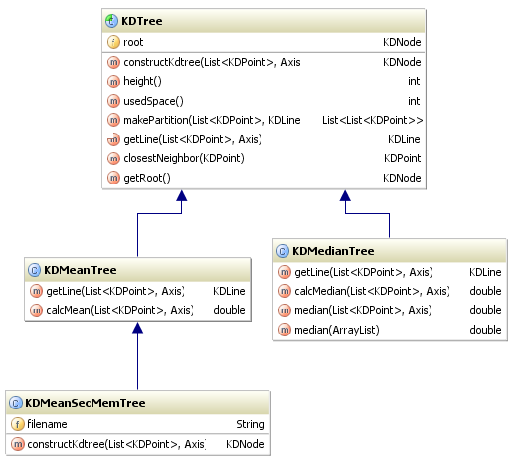
\includegraphics[scale=0.85]{img/TreeStructure.png}}
 \caption{UML para las clases que implementan la estructura}
\end{figure}

Por otro lado, son Nodos quienes guardan la información del árbol, pues este solo tiene un puntero al nodo raíz. Hay nodos de dos tipos, los internos guardan las rectas que particionan el espacio y las hojas guardan la información de los puntos, por lo que se tiene el siguente diagrama de clases:

\begin{figure}[ht!]
 \centering
\fbox{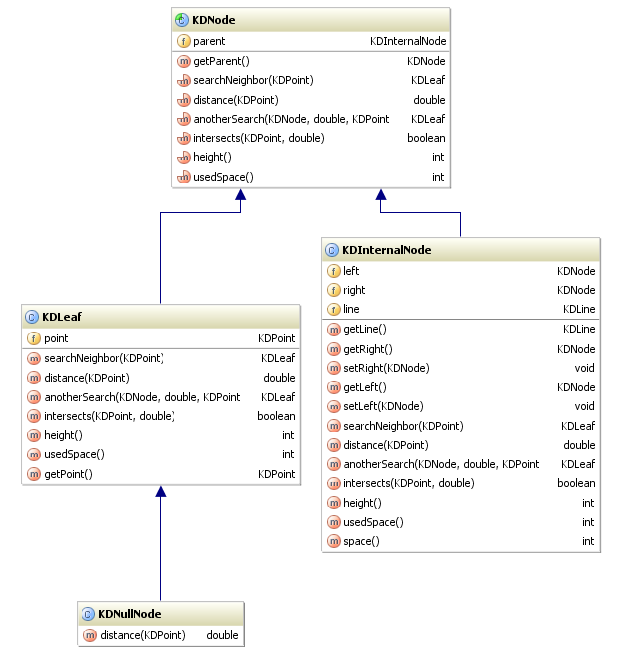
\includegraphics[scale=0.7]{img/nodeStructure.png}}
 \caption{UML para las clases que implementan los nodos}
\end{figure}
\newpage
Los nodos también son los responsables de recorrer el árbol durante las consultas, hacia los hijos y hacia el padre, además son los que calculan la intersección entre los sectores que delimitan y el círculo de consulta.

\subsection{Construcción del Árbol}

% -----Explicación de cómo funciona la construcción-------
La construcción se hace recursivamente, con caso base un conjunto de puntos de tamaño $1$. En cada fase se particiona el conjunto de acuerdo al criterio de mediana o media, intercalando el eje en cada nivel. El código es bastante simple y se presenta a continuación:
\begin{lstlisting}
public KDNode constructKdtree(List<KDPoint> points, Axis axis){
        if(points.size() == 1 ){
            return new KDLeaf(points.get(0));
        }
        KDLine line = getLine(points, axis) ; //This line depends on the Tree citeria
        List<List<KDPoint>> partition = makePartition(points,line);
        return new KDInternalNode(line,
                                  constructKdtree(partition.get(0),axis.negated()),
                                  constructKdtree(partition.get(1),axis.negated()));
    } 
\end{lstlisting}

Las diferentes implementaciones de getLine y el método partition pueden encontrarse en los anexos
% -------------------------------------------------------------

\subsection{Consultas de Vecino más cercano}

% -----Explicación de cómo funcionan las consultas------
Las consultas buscan descendentemente desde la raíz, el nodo del cuadrante que incluye al punto de consultas. Recordemos que el árbol crea una suerte de rejilla sobre el espacio, entonces la primera búsqueda le indica cual es el cuadrante del punto consultado y se calcula la distancia entre este y el punto del árbol de ese cuadrante.\\
Con esta distancia volvemos a subir por el árbol y vemos si el cuadrante que enmarca el otro hijo del nodo intersecta el circulo con centro el punto de consulta y radio la distancia que tenemos guardada. Así vamos subiendo y si encontramos alguna distancia mejor, la guardamos. Este comportamiento se registra en el siguiente código:
\newpage
\begin{lstlisting}
public KDPoint closestNeighbor(KDPoint q){
    KDLeaf currentBest = root.searchNeighbor(q);//looks for node, same sector than q
    double currentDistance = currentBest.distance(q);
    KDNode actual = currentBest.getParent();
    KDNode prev = currentBest;  
    
    while(actual!= null){
        KDLeaf temp = actual.anotherSearch(prev, currentDistance,q); //looks for a best fit
        if(temp.distance(q)<currentDistance){
            currentBest = temp;
            currentDistance = currentBest.distance(q);
        }
        prev = actual;
        actual = actual.getParent();
   }
   return currentBest.getPoint();
}
\end{lstlisting}

Los métodos searchNeighbot y anotherSearch se pueden encontrar en los anexos
% -------------------------------------------------------------
\newpage
\subsection{Diseño de los Experimentos}
Los experimentos consistieron en construir árboles KD con arreglos de puntos de tamaños sucesivamente más grandes (tamaño $2i$, $i\in\{10,...,20\}$ en las diferentes combinaciones de criterio de partición y de distribución de puntos y medimos su tiempo, la altura del árbol y la cantidad de espacio en memoria que utiliza. Luego a cada sabor de árbol le hacemos consultas y medimos el tiempo que toma en contestar. Cada experimento se repite las veces necesarias para que el error sea menor al 5\% (i.e., hasta que $\frac{stdv}{mean}\leq 0.05$). Para detalles de la implementación de la batería de experimentos, referirse al código fuente adjunto.

\newpage
\section{Resultados}
very successful

\newpage
\section{Conclusiones}
wow




% ============= ANEXOS =====================
\newpage
\section{Anexos}

\subsection{Merge function}
\begin{lstlisting}
static private int[] merge(int[] A, int[] B){
        int i=0, j=0, n=A.length+B.length;
        int[] res = new int[n];

        for(int k=0; k<n; k++){
           if(i<A.length && j<B.length){
               if(A[i]<=B[j]){
                   res[k] = A[i];
                   i++;
               }else{
                   res[k] = B[j];
                   j++;
               }
           } else if(i == A.length){ //si se acaban los elems de B
               for(;k<n;){
                   res[k] = B[j];
                   k++; j++;
               }
           }else{
               for(;k<n;){ //si se acaban los elems de A
                   res[k] = A[i];
                   k++; i++;
               }
           }
        }
        return res;
    }
}
\end{lstlisting}
\newpage
\subsection{Partition function}
\begin{lstlisting}
private static int partition(int[] A, int start, int end) {
    int index = start + new Random().nextInt(end-start);
    int pivot = A[index];
    int i = start, j = end;
    while(i<j){
        while(A[i] < pivot) i++;
        while(A[j] > pivot) j--;
        swap(A, i, j);
    }
    return i;
}
\end{lstlisting}

\subsection{Experimentos}
\subsubsection{Experimento 1}
\subsubsection{Experimento 2}
\subsubsection{Experimento 3}
\subsubsection{Experimento 4}

\subsection{Resultados}
\subsubsection{Resultado 1}
\subsubsection{Resultado 2}
\subsubsection{Resultado 3}
\subsubsection{Resultado 4}




% ============= FIN DE DOCUMENTO ==============
\end{document}

% % ················ IMAGEN ·················
% \begin{figure}[ht!]
% \centering
% \fbox{\includegraphics[scale=0.6]{img/torneo.png}}
% \caption{Torneo}\label{torneo}
% \end{figure}
% %··········································

% % ················ IMAGEN DOBLE ·················
% \begin{figure}[ht!] \centering
% \subfloat[Hola]{\includegraphics[scale=0.44]{img/holaquetal.png}}
% \subfloat[Que tal]{\includegraphics[scale=0.45]{img/holaquetal1.png}}
% \caption{Holaquetal}\label{holaquetal}
% \end{figure}
% %··········································